\subsection{Audio Generation based on Video}
% \dq{@yutao, james, miles}

Our video-to-audio(V2A) module is designed to enhance generated video content by incorporating synchronized sound effects and contextually appropriate background music. Within the conventional film production pipeline, Foley sound design constitutes an integral component, significantly contributing to the auditory realism and emotional depth of visual media. However, the creation of Foley audio is both time-intensive and demands a high degree of professional expertise. With the advent of an increasing number of text-to-video (T2V) models, most of them lack the corresponding foley generation capabilities, thereby limiting their ability to produce fully immersive content. Our V2A module addresses this critical gap by autonomously generating cinematic-grade foley audio tailored to the input video and textual prompts, thus enabling the synthesis of a cohesive and holistically engaging multimedia experience.

\subsubsection{Data }
Unlike text-to-video (T2V) models, video-to-audio (V2A) models have different requirements for data. As mentioned above, we constructed a video dataset comprising of video-text pairs. However, not all data in this dataset are suitable for training the V2A model. For example, some videos lack an audio stream, others contain extensive voice-over content or their ambient audio tracks have been removed and replaced with unrelated elements. To address these challenges and ensure data quality, we designed a robust data filtering pipeline specifically tailored for V2A training.

First, we filter out videos without audio streams or those in which the silence ratio exceeds 80\%. Next, we employ a frame-level audio detection model, like \cite{Hung2022}, to detect speech, music, and general sound in the audio stream. Based on this analysis, we classify the data into four distinct categories: \textit{pure sound}, \textit{sound with speech}, \textit{sound with music}, and \textit{pure music}. Subsequently, to prioritize high-quality data, we train a model inspired by CAVP \cite{luo2024diff} to compute a visual-audio consistency score, which quantifies the alignment between the visual and auditory components of each video. Using this scoring system in conjunction with the audio category labels, we systematically sample portions of data from each category, retaining approximately 250,000 hours from the original dataset for pre-training. For the supervised fine-tuning stage, we further refine our selection, curating a subset of millions of high-quality clips~(80,000 hours).

For feature extraction, we use CLIP \cite{clip} to obtain visual features at a temporal resolution of 4 fps and subsequently resample these features to align with the audio frame rate. To generate captions, we employ \cite{haji2024taming} as the sound captioning model and \cite{doh2023lp} as the music captioning model. When both sound and music captions are available, we merge them into a structured caption format, following the approach detailed in \cite{polyak2024movie}.

\subsubsection{Model}
Just like the above-mentioned text-to-video model, our video-to-audio generation model also adopts a flow-matching-based diffusion transformer (DiT) as its architectural backbone. The detailed design of the model is depicted in Figure \ref{fig:audio-gen}, illustrating a transition from a triple-stream structure to a single-stream DiT framework.

The model operates within a latent space encoded by a variational autoencoder (VAE) trained on mel-spectrograms. Specifically, the audio waveform is first converted into a 2D mel-spectrogram representation. This spectrogram is subsequently encoded into a latent space using a pretrained VAE. For feature extraction, we leverage pretrained CLIP \cite{clip} and T5 \cite{raffel2020exploring} encoders to independently extract visual and textual features, respectively. These features are subsequently projected into the DiT-compatible latent space using independent linear projections followed by SwiGLU activation, as depicted in Figure \ref{fig:audio-gen}.

To effectively integrate multimodal information, we incorporate stacked triple-stream transformer blocks, which independently process visual, audio, and textual modalities. These are later followed by single-stream transformer blocks to ensure seamless fusion and alignment across modalities. This design enhances the alignment between audio-video and audio-text representations, facilitating improved multimodal coherence.

Once the latent representation is generated by the diffusion transformer, the VAE decoder reconstructs the corresponding mel-spectrogram. Finally, the mel-spectrogram is converted back into an audio waveform using a pre-trained HifiGAN vocoder \cite{kong2020hifi}. This framework ensures a high-fidelity reconstruction of audio signals while maintaining strong multimodal alignment.

\begin{figure}[t]
    \centering
    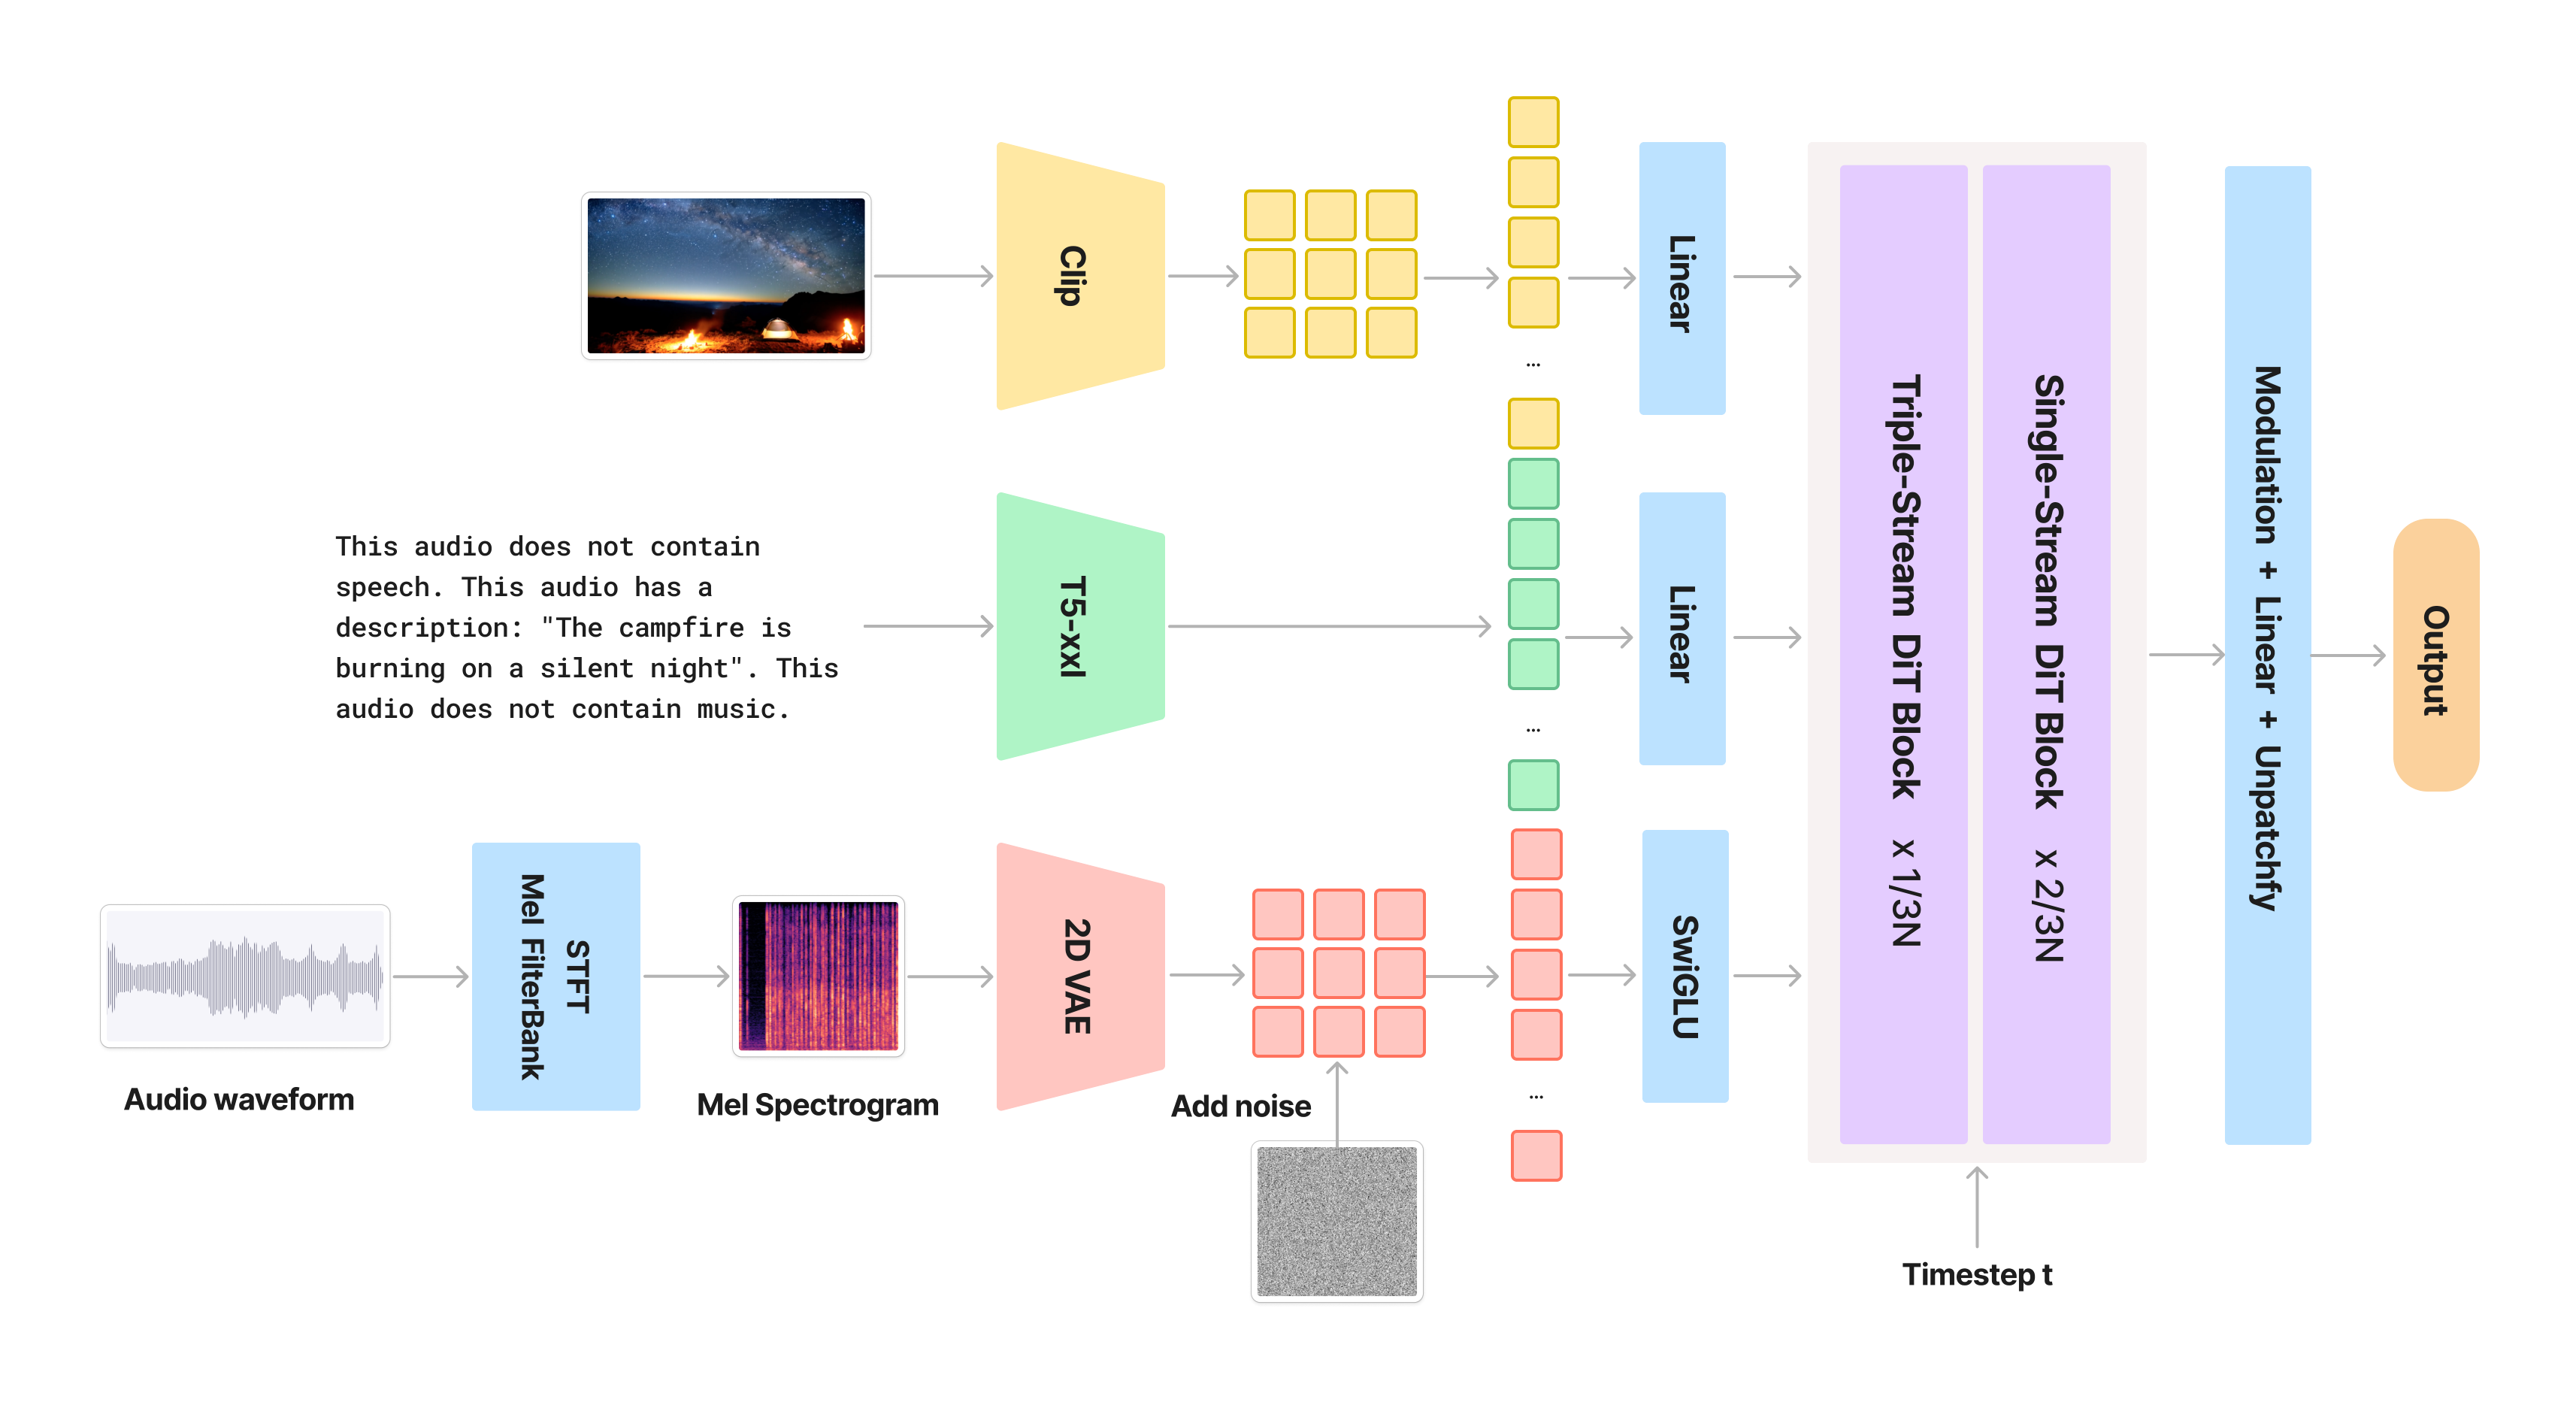
\includegraphics[width=0.9\linewidth]{figures/vt2a_arch.png}
    \caption{The architecture of sound effect and music generation model. }
    \label{fig:audio-gen}
\end{figure}